\documentclass[01pt]{article}

\usepackage[utf8]{inputenc}
\usepackage{graphicx}
\usepackage{amssymb, amsmath, amsthm}
\usepackage{bbm}
\usepackage{enumitem}   
\linespread{1.15}
\usepackage{titlesec}
\usepackage{hyperref}
\usepackage{chngpage}
\usepackage{wrapfig}
\usepackage[margin=1.0in]{geometry}


%%%%%%%%%%%%%%%%%%%%%%
\usepackage{fancyhdr}
\pagestyle{fancy}
\lhead{MA 703: HW2}
\rhead{Benjamin Draves} 


\usepackage[backend=biber]{biblatex}
\addbibresource{ref.bib}
\AtNextBibliography{\footnotesize}
\titlespacing*{\section}{0pt}{1ex}{1ex}

\parskip = 0.1in
\newcommand{\bvar}[1]{\mathbf{#1}} 

\begin{document}

\section{Summary of SWU4 Study}

The \textit{SWU4} dataset is a collection of neurological images (anatomical, resting state fMRI, and DTI) of 227 students attending Southwest China Normal University. 
Participants were recruited from the SWU campus and were imaged twice roughly one year apart. 
The data was made public by the Consortium for Reliability and Reproducibility \cite{Zuo2014} and later expanded as part of the 
Southwest University Longitudinal Imagining Multimodal (SLIM) dataset. 
The data used in this report was accessed through Nuerodata's \textit{MRI-Cloud} project\footnote{http://neurodata.io/} which produces connectomes- network representations of brain structure and function- from neurological imaging data using NeuroData's MRI to Graph (\textit{NDMG}) pipeline. 
\textit{NDMG} was constructed in an attempt to remove the need to construct custom pipelines for processing imagining data which consequently may jeopardize the reproducibility of studies that rely on these custom tools. 
We refer the reader to Appendix B of Kiar et al.\cite{Kiar188706} for a complete description of the methods used in each stage of this pipeline.

In this report, we restrict our analysis to DTI (diffusion tensor imaging) images. 
DTI is a particular type of diffusion Magnetic Resonance Imaging (dMRI) that has been used to map the diffusion of water molecules within neural tissue. 
By identifying these diffusion patters, DTI can be used in identifying systems, called \textit{nerve tracts}, that connect different nuclei of the central nervous system\cite{Soares2013}. 
Vertices in this area are defined according to a practitioner specified \textit{parcellation} - a mapping that assigns regions, called \textit{voxels}, of the brain to vertices of the network based on functional, anatomical, or spatial features.
Here, we use the CC200 parcellation \cite{Craddock2012} which defines a vertex set $V$ of size $N_V = 200$.
Edge weights are then defined according to the number of tracts that connect these regions. 
In particular, the edge weight between vertices $v_i$ and $v_j$ is given by 
\begin{align}
    w(v_i, v_j) = \sum_{u\in N(v_i)}\sum_{w\in N(v_j)} I(F_{u,w})
\end{align}
where $N(v) = \{\text{voxels in $v$}\}$ is the set of voxels assigned to vertex $v$ by the parcellation and where $F_{u,w}$ is true if there is a tract that connects voxel $u$ and voxel $w$. 
In this definition, we implicitly define the edge set $E$ to be the pair vertices that share tracts between voxels in their respective neighborhoods. 
The \textit{NDMG} pipeline provides these network summaries of the DTI images for each of the 227 students at two imaging sessions, resulting in 454 network graphs. In addition, the \textit{SWU 4} dataset provides phenotype information on the participants (e.g. Age, Sex) and the CC200 parcellation provides vertex attributes (e.g. vertex coordinates in the stereotaxic-coordinate system, region of the brain, amount of tissue found in each $N(v_i)$). 
For an example of one such network produced by the \textit{NDMG} pipeline, see Figure \ref{fig:brain}. 

%\begin{figure}[h!]
\begin{wrapfigure}{R}{0.5\textwidth}
    \centering
    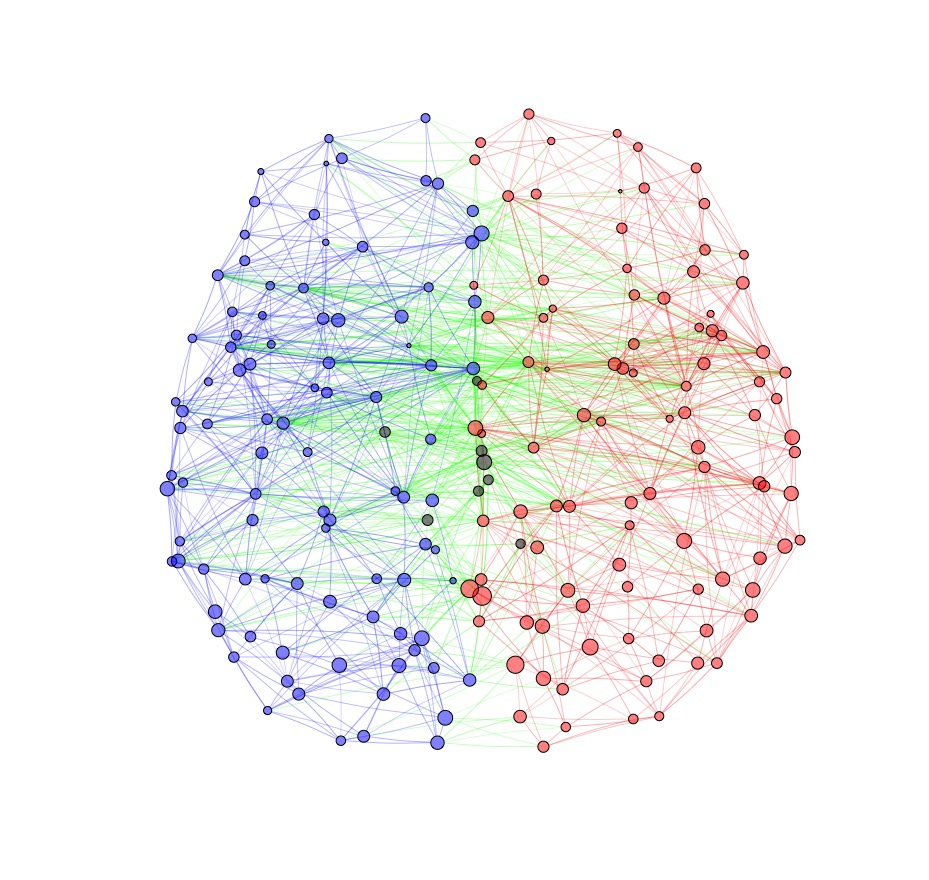
\includegraphics[height = 6cm, width = 6cm]{figures/Brain.jpeg}
    \caption{Subject 0025629's first session brain network graph as produced by the \textit{NDMG} pipeline using DTI imaging. Vertices are colored according to the anatomical region (left - blue, right - red, unknow - grey). Edges are colored by anatomical region if both incident nodes fall in the same region and are colored green otherwise. Size of vertices are proportional to the amount of tissue found in each $N(v_i)$.}
    \label{fig:brain}
\end{wrapfigure}
%\end{figure}

\section{Research Objectives}

Oftentimes, it is of interest to attribute different functional tasks to particular anatomical regions of the brain.
Indeed, work has shown that the left and right side of the brain undertake very different functional roles \cite{Corballis2014}. 
While functional MRI data attempts to capture the functional organization of the brain, DTI more readily captures structural organization. 
In order to support these functional differences, one may hypothesize that this left-right division may also play a role in the structural organization of the brain. 
Indeed, I hypothesize that the induced subgraph of vertices in the left and right side of the brain will be more cohesive than the graph-wide cohesion. 

There are several measures for network cohesion available to test this hypothesis.
In particular, we are interested a statistic which captures the propensity of vertices to collect more within anatomical region than between anatomical regions while also incorporating the weighted nature of these network graphs. 
One such statistic that satisfies these requirements is Barrat's clustering coefficient \cite{Barrat2004}. 
Roughly, this clustering coefficient measures the probability adjacent vertices of a vertex of interest are also connected while weighting by the edge weighes in the graph. 
The statistic is given by 
\begin{align}
    C^{w} = \frac{1}{N_v}\sum_{i=1}^{N_v}\left\{\frac{1}{s_i(k_i - 1)}\sum_{j,h\neq i}\left(\frac{w_{ij}+w_{ih}}{2}a_{ij}a_{jh}a_{ih}\right)\right\}
\end{align}
where $w_{ij}$ is the edge weight between vertex $i$ and $j$, $a_{ij}$ is the binary variable indicating an edge between vertex $i$ and $j$, $k_i$ is the degree of vertex $i$, and $s_i = \sum_{j\neq i}w_{ij}a_{ij}$ is the \textit{strength} of vertex $i$. 
As in the standard clustering coefficient, each summand counts the number of closed triangles within the neighborhood of vertex $i$ but weights this value by the average weight found on incident edges. 
The normalization term $s_i(k_i-1)$ is the maximum number of triangles vertex $i$ can be in times the maximum edge weight which ensures that each summand falls within the unit interval. 
Lastly, we take the mean over full network to measure average clustering within the network. 

If our hypothesis - that the left and right brain are more likely to have collections of vertices that cluster together to support functional behavior - is true, than we expect to see higher clustering coefficients for the induced subgraph of vertices in the left and right brain than across the full brain. 
If we only consider a single brain network, this will produce a simple three number summary. 
In order to more robustly explore if there is a difference in the clustering coefficient for different regions of the brain, one may construct a generative probability model in order to construct an appropriate reference distribution to compare this three number summary. 
Constructing a generative model that mimics the structure of the brain is a daunting task. 
Instead, we will collect this three number summary across all 454 networks in the \textit{SWU 4} study and compare the distributions of the observed clustering coefficients. 

By analyzing our first hypothesis in this way, we are implicitly assuming that each statistic collected, and therefore each network graph, is independent. 
However, we know that each student was imaged twice which immediately violates this assumption. 
Moreover, it may be the case that brain scans are not be independent across relevant phenotype subgroups such as Age and Sex. 
This leads to our second research question; is there a difference in the structure of the brain, as measured by Barrat's clustering coefficient, between phenotype subgroups? 
We analyze this research question in a similar way as we did as our first hypothesis, this time comparing distributions of the clustering coefficient for the left, right, and full brain between Age, Sex, and imaging session. 
If there is a difference between these subgroups, we expect to see a difference in the distribution of the clustering coefficients. 

Finally, we look to investigate if their is a difference between structural centrality and physical centrality of the brain.
For example, it may be the case that central vertices to the DTI network graph do not lie in the center of the brain. 
Leveraging the fact that the DTI networks are embedded into $\mathbb{R}^3$, we can compare the physical center of the brain to the ``center" of each observed network graph. 
Let $p_1, p_2, \ldots, p_{200}\in\mathbb{R}^{200}$ be the physical locations of the vertices in the CC200 parcellation. 
We consider the physical center, denote $P_{PC}$, as the mean of these points. 
To measure structural centrality, we propose the following metric based on the eigen-centrality of the graph.
Recall the eigencentrality defines the centrality $\bvar{x}_i$ of vertex $i$ by the recursive definition $\bvar{x}_i = t^{-1}\sum_{j\sim i}\bvar{x}_j$ where $t$ is the number of neighbors of $i$.   
In order to incorporate the weighted nature of the graph,
let $\bvar{x}$ be the eigenvector corresponding to the largest eigenvalue of the \textit{weighted}-adjacency matrix $\bvar{W}$. 
Then $\bvar{x}_i$ measures the weighed eigen-centrality of vertex $i$.
Next, define the \textit{normalized} eigen-centrality $\tilde{\bvar{x}} = \bvar{x}/\|\bvar{x}\|_1$ so that $1 = \sum_{i=1}^{N_v}\tilde{\bvar{x}}_i$. 
From here we define the structural center $P_{SC}$ as the weighted sum of the $p_i$ with respect to $\tilde{\bvar{x}}_i$.
In this way, the weights encode the centrality of each position and the weighed sum gives a centrality measure based instead on the eigen-centrality of each physical location. 
Formally, we define two measures of centrality in this report
\begin{align}
    P_{PC} = \sum_{i=1}^{N_v}\frac{p_i}{N_v}\hspace{4em}P_{SC} = \sum_{i=1}^{N_v}\tilde{\bvar{x}}_ip_i
\end{align}

Notice that $P_{PC}$ is fixed with respect to the parcellation.
As we have 227 individuals and consequently 454 brain images, $P_{SC}$ will vary with respect to the DTI image. 
We will therefore collect $\{\hat{P}_{SC}^{(i)}\}_{i=1}^{454}$ for each brain image. 
Having this cloud of points in $\mathbb{R}^{3}$, we will then construct multivariate t-distribution confidence ellipses and compare $P_{PC}$ to these intervals. 


\section{Results \& Conclusion}

\begin{figure}
\begin{adjustwidth}{-.5in}{-.5in}
    \centering
    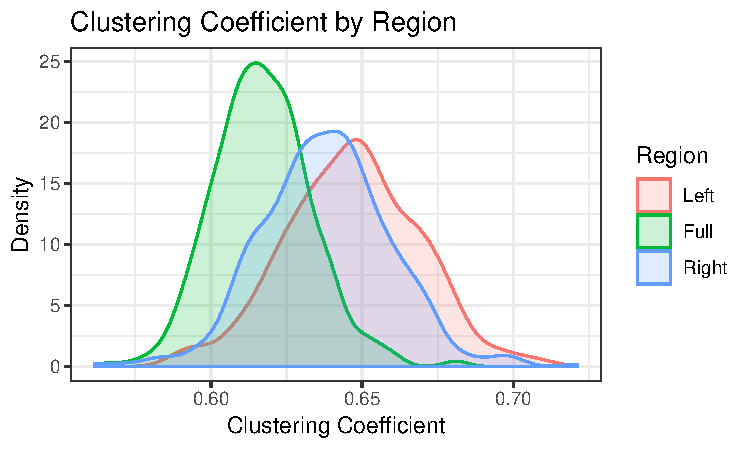
\includegraphics[width = .5\textwidth, height = .3\textwidth ]{figures/clustering_coef_region_comp.pdf}
    \caption{The observed distribution of Barrat's clustering coefficient by region. It appears that vertices in the left and right side form slightly more cohensive clusters than collections of vertices in the full network. }
    \label{fig:CC_by_region}
\end{adjustwidth}
\end{figure}

We first investigate the results pertinent to testing the first hypothesis. 
Plotted in Figure \ref{fig:CC_by_region} is the distribution of the observed clustering coefficients by each region of the brain. 
In green is the full brain clustering coefficients while the red and blue are the clustering coefficients from the left and right brain. 
It appears that the distribution of the left and right brain are shifted to the right when compared to the full brain. 
Indeed, the 95\% empiracle interval of the full brain was $(0.588, 0.651)$ as compared to the left brain $(0.603,0.690)$ and right brain right side $(0.597,0.678)$
While these intervals largely overlap, they do appear to shifted slightly as evident by Figure \ref{fig:CC_by_region} as well as the change in the center of these intervals. 
We also note that it appears the variances of these distributions is higher among the left and right brains than the full brain. 
This observation is also supported by increased width of left and right brain intervals given above. 
Therefore, we believe this serves as exploratory evidence to suggest that vertices may tend to cluster slightly more cohesively within anatomical regions of the brain than across the full brain. 



\begin{figure}[h!]
   \begin{adjustwidth}{-.5in}{-.5in}
    \centering
    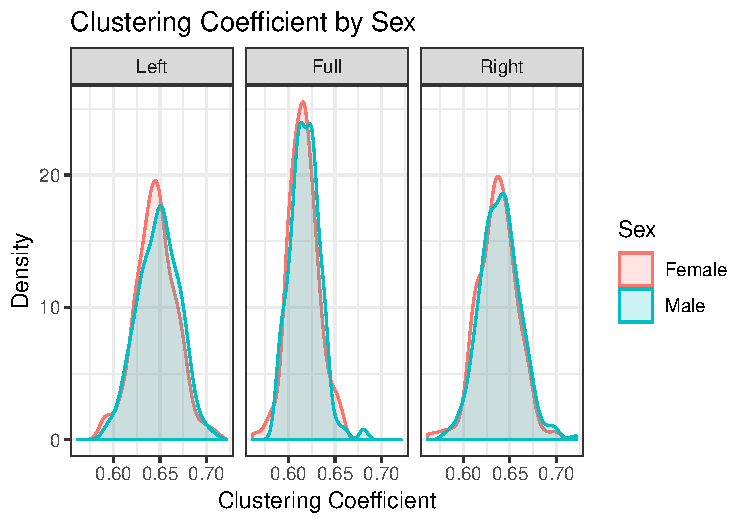
\includegraphics[width = .4\linewidth, height = .3\linewidth]{figures/clustering_coef_male_versus_female.pdf}
    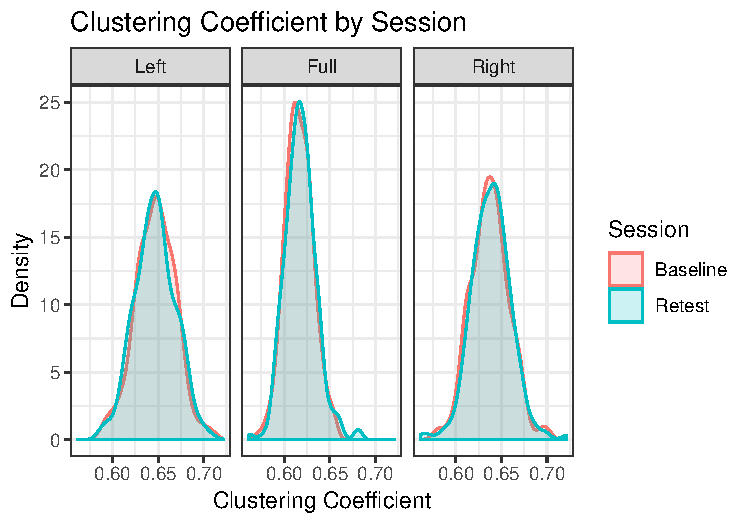
\includegraphics[width = .4\linewidth, height = .3\linewidth]{figures/clustering_coef_session_by_session.pdf}\\
    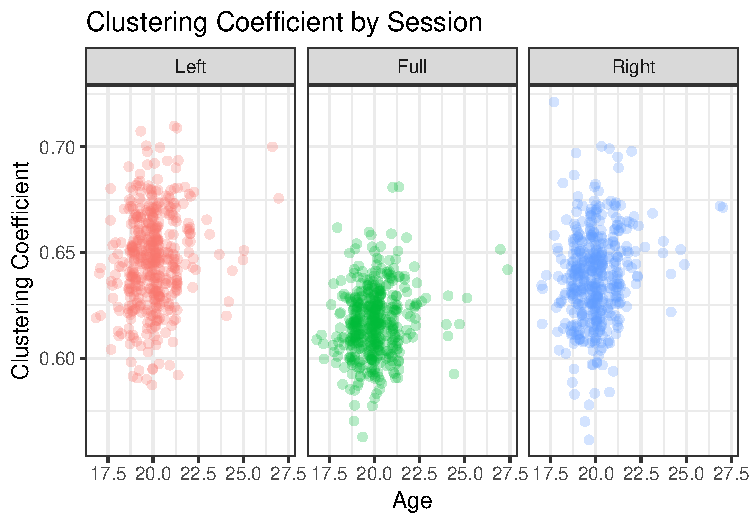
\includegraphics[width = .45\linewidth, height = .3\linewidth]{figures/clustering_coef_by_age.pdf}
    \caption{\textit{Top left}: The distribution of clustering coefficient for the left brain (left), full brain (center), and right brain (right) by Sex (Male \& Female). \textit{Top right}: The distribution of clustering coefficient by session (Baseline \& Retest). \textit{Bottom}: A jittered scatter plot of clustering coefficient by age. In all three plots it appears that the clustering coefficient is independent of each independent variable.}
    \label{fig:CC_by_phenotype}
    \end{adjustwidth}
\end{figure}

Next we turn to analyzing our second hypothesis and hope to understand if there is a difference in the clustering of nodes within the left, right, or full brain between Sex, Age, or session number. 
Three plots illuminating this questions are provided in Figure \ref{fig:CC_by_phenotype}. 
In the top left panel is a density plot of the clustering coefficient for the left, full, and right brain for both Male and Female participants. 
Immediately, it is clear that there is very little disagreement between the two distributions for any region of the brain. 
Indeed, it is almost difficult to distinguish the two distributions in the same plot. 
Similarly, in the top right panel, the clustering coefficient for each region of the brain is compared across imaging session one and two. 
Again, it appears that there is little to no discrepancies between these distributions. 
Lastly, we plot the observed clustering coefficients for each region of the brain against the age of the participant. 
As no clear pattern emerges in this plot, these two variables appear to be uncorrelated.
These results suggest that the propensity of vertices in the network to cluster together - in any region of the brain - does not differ between imaging session, Sex, or Age. 

Finally, we look to investigate if there a difference between physical centrality as measured by $P_{PC}$ as compared to the estimated structural centers $\hat{P}_{SC}$. 
Consider Figure \ref{fig:Centrality} for the results of this analysis. 
Plotted in blue are the physical locations of the vertices $\{p_i\}_{i=1}^{200}$. 
In order to visualize these points in $\mathbb{R}^2$, we plot their projections onto the $xy$-plane (left), the $xz$-plane (center), and the $yz$-plane (right).
The blue X marks the center of these points, $P_{PC}$.
The red points are the appropriate projections of each $\{\hat{P}_{SC}\}_{i=1}^{200}$ and the red dashed ellipses are the estimated $95\%$ multivariate t-confidence intervals visualized in each plane. 


\begin{figure}[h!]
   \begin{adjustwidth}{-.5in}{-.5in}
    \centering
    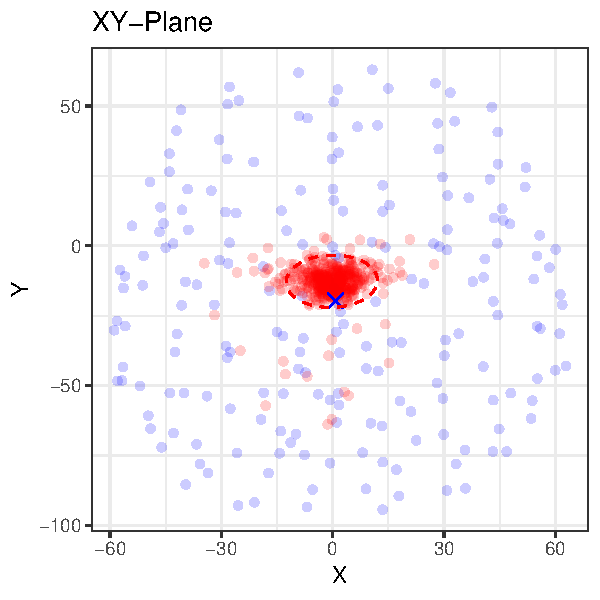
\includegraphics[width = .25\linewidth]{figures/centrality_xy.pdf}
    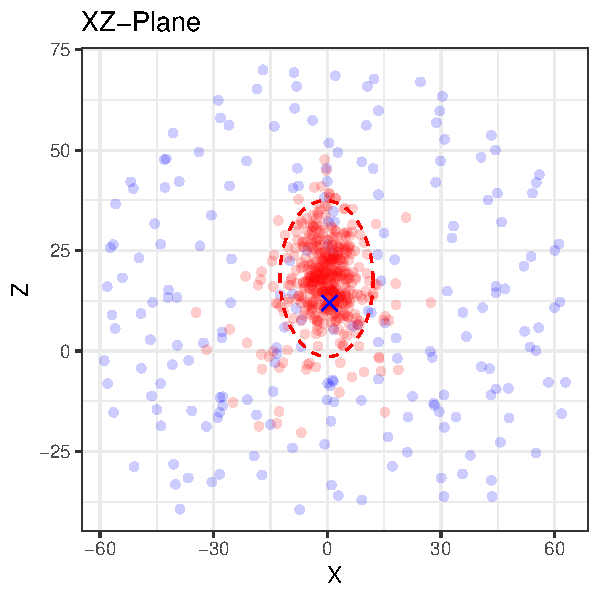
\includegraphics[width = .25\linewidth]{figures/centrality_xz.pdf}
    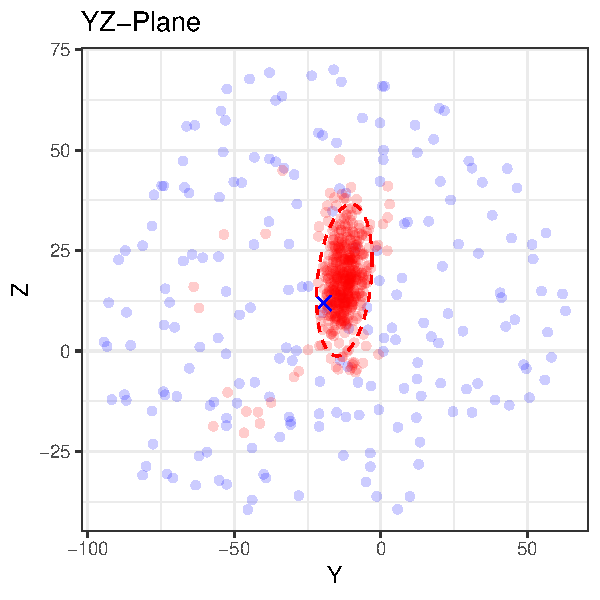
\includegraphics[width = .25\linewidth]{figures/centrality_yz.pdf}
    \caption{Plot of the vertex locations (blue points), the parcellation center (blue X), and estimated centers (red points). The dashed red lines are estimated 95\% multivariate t confidence intervals. These points were projected into the XY-plane (left), XZ-plane (center), and the YZ-plane (right) for visualization. }
    \label{fig:Centrality}
    \end{adjustwidth}
\end{figure}

From the figure, we first note that there is very little variability along the y axis (back to front), followed by variability on the x axis (ear to ear), while the most variability existed among the z axis (top to bottom). 
Therefore, there was more consistent agreement of centrality from the $\hat{P}_{SC}^{(i)}$ along the y-axis than any other. 
Also from the figure, each confidence ellipse contains the central $P_{PC}$ point. 
This suggests that the central of the CC200 parcellation, $P_{PC}$, coincides with our estimate of structural centrality $P_{SC}$. 

These figures and statistics help elicit insight into our stated research objectives. 
Figure \ref{fig:CC_by_region} suggests that there may be a slight tendency of vertices to cluster more within anatomical regions than across anatomical regions of the brain.
Moreover, Figure \ref{fig:CC_by_phenotype} suggests this phenomena is independent of the participants Sex, Age, or which session the image was taken. 
Finally, Figure \ref{fig:Centrality} suggests that the physical center of the brain coincides with the center of the structural organization of the brain.
Results like these can aid in our understanding of the structure of the brain and how that structure relates to its function. 


\printbibliography
\nocite{*}


\end{document}






















